\documentclass[fleqn]{homework}

\student{Stephen Brennan (smb196)}
\course{EECS 440}
\assignment{Programming 2}
\duedate{October 8, 2015}

%\usepackage{mathtools}
%\usepackage{graphicx}

\begin{document}
  \maketitle

  \section{Implementation Commentary}

  Unlike the decision tree implementation, artificial neural networks readily
  suggest a matrix based implementation, which can be done using more native
  NumPy code and less pure Python code, which makes the overall implementation
  fairly efficient.  I chose to express each layer as a matrix, where each
  column represents the weights for a unit in that layer.  This means that
  feeding a matrix $X$ through a layer $W$ is as simple as computing
  $X \cdot W$, followed by computing the sigmoid function of the result.
  Training can be accomplished using elementwise arithmetic on these matrices,
  using NumPy's broadcasting capabilitiess to account for differences in matrix
  sizes.

  I use several single letter indexing variables to denote sizes, both in
  comments and in code.  Here are the conventions I used throughout the code,
  which should make understanding the code (especially the gradient
  computations) easier.

  \begin{itemize}
  \item Where $k$ is used as a variable, it refers to the number of examples
    provided.
  \item Where $n$ is used as a variable, it refers to the number of inputs to a
    layer.  When talking about the first layer, this is the number of
    attributes.  For the second layer, this is the number of units it the first
    layer, etc.
  \item Where $m$ is used as a variable, it refers to the number of units in a
    layer (which is also the number of outputs of that layer).
  \item Where $p$ is used as a variable, it refers to the number of units in the
    subsequent layer.
  \end{itemize}

  Also, this implementation strategy is only valid since each layer is
  completely connected to each subsequent layer.  If the network topology were
  different, I would have to use a different (and probably much slower)
  implementation strategy.

  Finally, the implementation should generalize well into architectures with any
  number of hidden layers (including 0).  The constructor always creates
  ``rectangular'' hidden layers, but it would only take slight modifications to
  the constructor to allow any number of units in any hidden layer.

  \section{Questions}

  \begin{problem}{a}
    \begin{question}
      What is the area under ROC of the ANN with no hidden units on each
      dataset? Set the weight decay coefficient $\gamma = 0$, and train to
      convergence. This approximates the perceptron, which uses a step function
      instead of a sigmoid. How does this compare to the decision stump/tree
      results in the previous assignment?
    \end{question}

    \begin{tabular}{|lr|rrrr|}
      \hline
      Dataset & $\epsilon$ & Accuracy & Precision & Recall & AUC \\
      \hline
      Voting & 0.01 & $0.986 \pm 0.009$ & $0.995 \pm 0.010$ & $0.974 \pm 0.016$ & 0.994 \\
      Volcanoes & 0.01 & $0.806 \pm 0.051$ & $0.760 \pm 0.063$ & $0.635 \pm 0.252$ & 0.719\\
      Spam & 0.2 & $0.663 \pm 0.013$ & $0.632 \pm 0.011$ & $0.991 \pm 0.012$ & 0.525 \\
      \hline
    \end{tabular}

    \vspace{4mm}

    Unfortunately, there was no ``solid'' definition of convergence that I could
    use in my code.  So, I defined convergence as: ``all elements of the
    gradient are less than $\epsilon$.''  This worked alright, but the amount of
    time my ANN took to converge varied wildly, even across folds.  My attempts
    to get the \textit{spam} dataset to converge with $\epsilon=0.01$ never
    completed.  $\epsilon = 0.2$ was the first value that I obtained any
    convergence for (and it converged after about 1000 iterations on each fold).
    Meanwhile, \textit{volcanoes} took in the tens of thousands of iterations to
    converge at $\epsilon = 0.01$, and \textit{voting} took anywhere from a few
    hundred to several thousand at the same $\epsilon$.
  \end{problem}

  \begin{problem}{b}
    \begin{question}
      For \textit{volcanoes} and \textit{spam}, and explore how the AROC changes
      as learning iterations are increased. Fix the number of hidden units to 5
      and $\gamma = 0.01$ for these experiments. Plot AROC results for at least
      three values of learning iterations evenly spaced between 100 and
      10,000. Compare your results to the “perceptron” in part
      \textbf{(a)}. Does the introduction of hidden units lead to improved
      accuracy? How many iterations does this ANN need to converge compared to
      the “perceptron”?
    \end{question}

    \begin{tabular}{|lrr|}
      \hline
      Dataset & Iterations & AUC \\
      \hline
      Volcanoes & 100 & 0.671 \\
      Volcanoes & 500 & 0.758 \\
      Volcanoes & 1000 & 0.679 \\
      Volcanoes & 2000 & 0.659 \\
      Volcanoes & 5000 & 0.653 \\
      Volcanoes & 10000 & 0.672 \\
      Spam & 100 & 0.497 \\
      Spam & 500 & 0.506 \\
      Spam & 1000 & 0.506 \\
      Spam & 2000 & 0.507 \\
      Spam & 5000 & 0.508 \\
      Spam & 10000 & 0.491 \\
      \hline
    \end{tabular}

    The table above shows the results from my experimenting by varying the
    number of iterations, and the data are plotted in Figure~\ref{fig:part-b}.
    I'm not sure whether the \textit{volcanoes} 500 iteration data point is an
    outlier, or whether 500 iterations is some sort of ``sweet spot'' for this
    setup (I would imagine it is more likely to be an outlier).  In any case,
    adding the 5 unit hidden layer doesn't improve ROC over the ``perceptron''
    much except in that data point.  It's a but unfortunate to see that there
    isn't a reliable upward trend either.

    \begin{figure}
      \centering
      \caption{AUC vs training iterations, on both volcanoes and spam (part b).}
      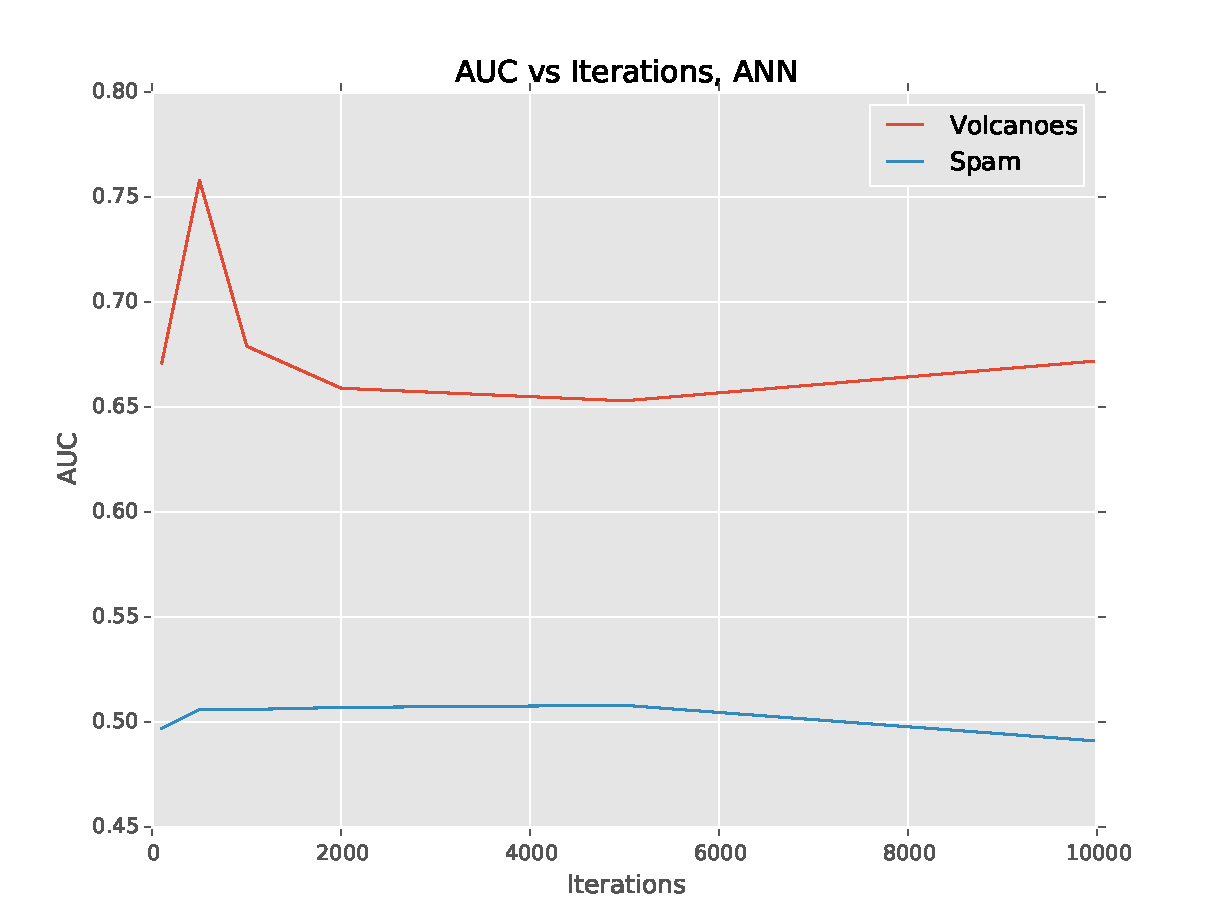
\includegraphics[width=0.7\textwidth]{partb.pdf}
      \label{fig:part-b}
    \end{figure}
  \end{problem}

  \begin{problem}{c}
    \begin{question}
      Explore how the AROC changes as the number of hidden units are varied on
      volcanoes and voting.  Plot AROC results for at least three values of
      hidden units evenly spaced between 3 and $f$, where $f$ is the number of
      input units. Set $\gamma=0.01$ and the learning iterations to $100f$, with
      a minimum of 10,000.  Compare the ROC and training times to the results in
      parts \textbf{(a)} and \textbf{(b)}. Warning: This experiment may take a
      long time to run.
    \end{question}

    Since \textit{voting} only has 11 attributes, I set it to 10,000 iterations.
    While I wanted to get \textit{volcanoes} to the full 22,600 iterations
    corresponding to its 226 attributes, I wasn't able to get the 226 hidden
    unit trial to complete in a reasonable amount of time.  So, I set
    \textit{volcanoes} to 10,000 iterations as well.

    Plots for my results are provided as Figures~\ref{fig:part-c-volcanoes}
    and~\ref{fig:part-c-voting}.  The plot for \textit{volcanoes} looks like an
    upside-down volcano, which is unfortunate, because I can't really draw too
    many conclusions from it.  The plot of \textit{voting} is similarly
    uninformative.

    \begin{figure}
      \centering
      \caption{AUC vs Hidden Units, Volcanoes (part c)}
      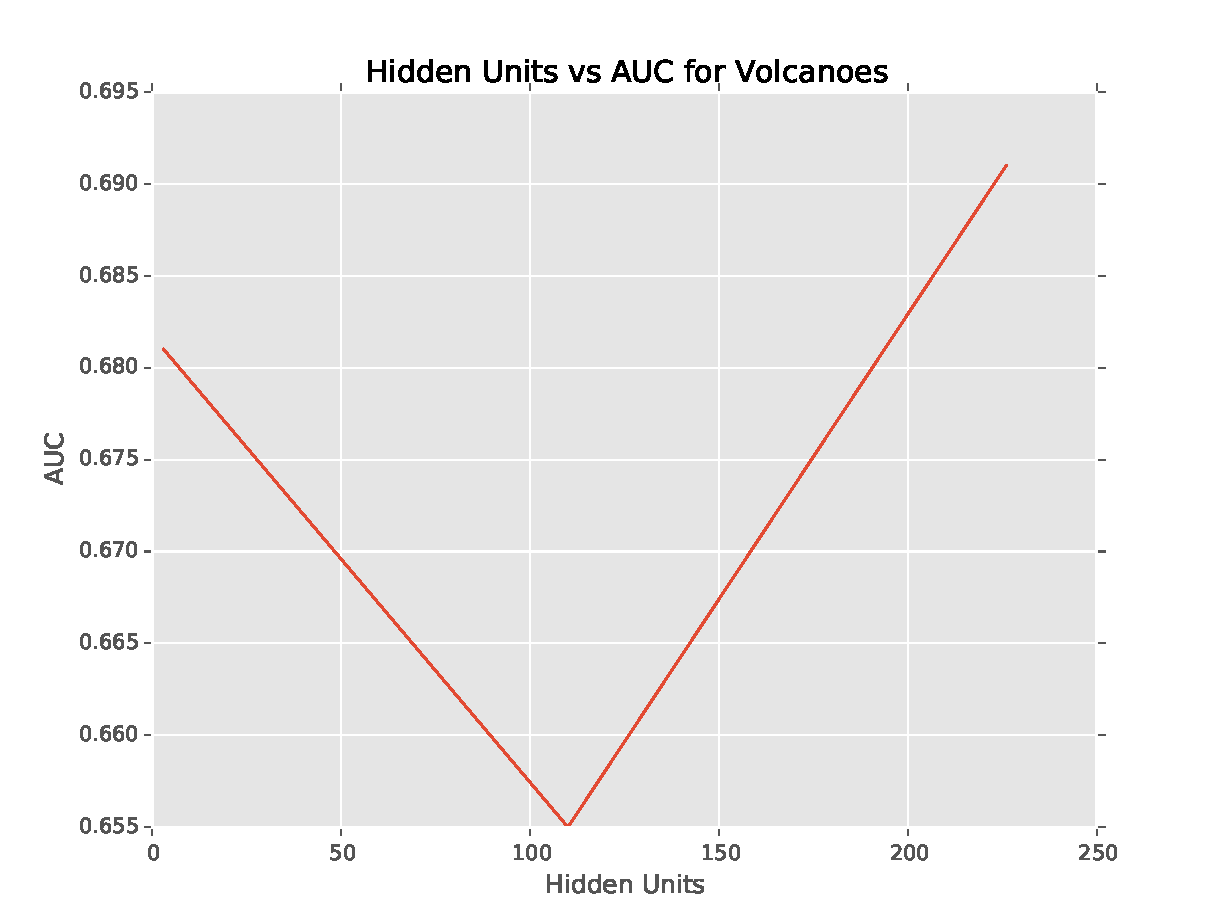
\includegraphics[width=0.7\textwidth]{partc-volcanoes.pdf}
      \label{fig:part-c-volcanoes}
    \end{figure}

    \begin{figure}
      \centering
      \caption{AUC vs Hidden Units, Voting (part c)}
      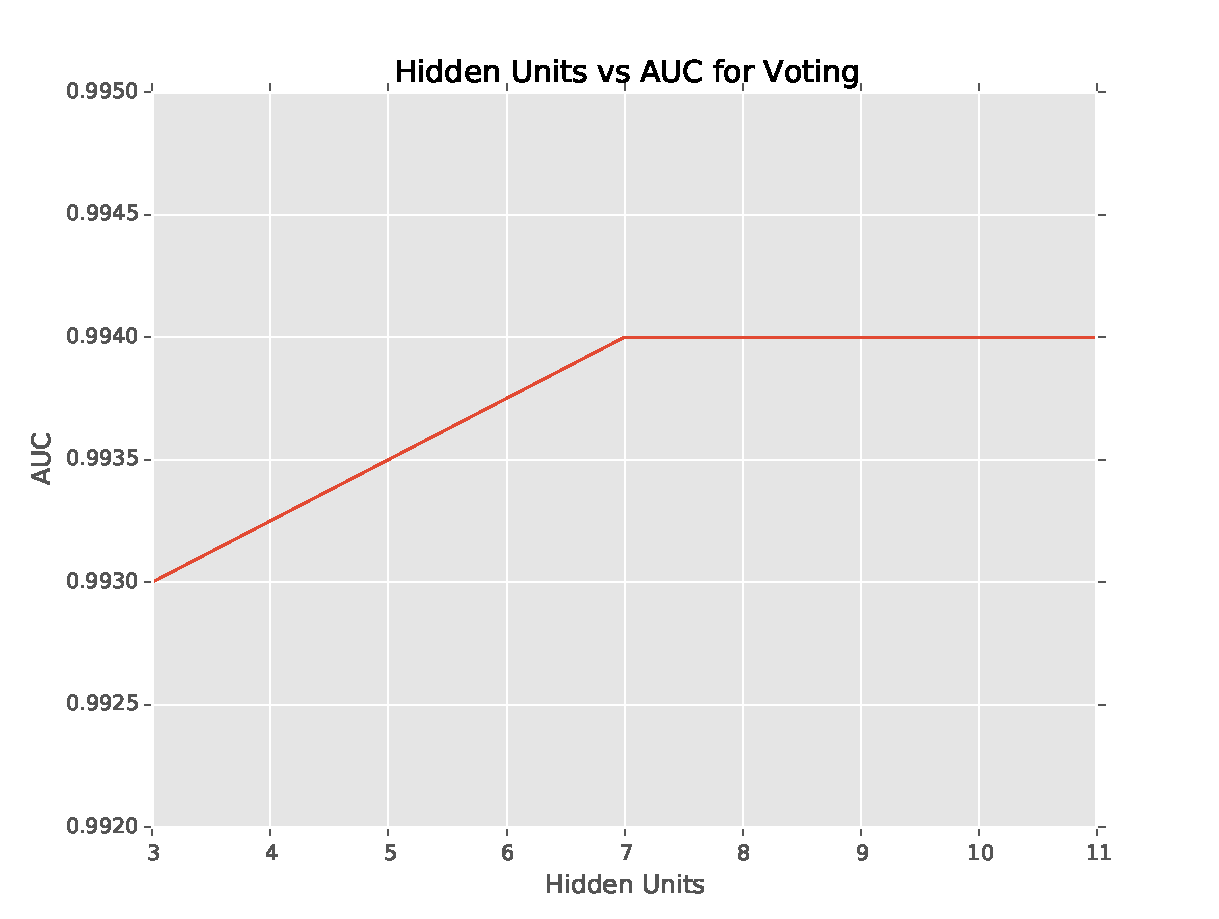
\includegraphics[width=0.7\textwidth]{partc-voting.pdf}
      \label{fig:part-c-voting}
    \end{figure}

    \begin{tabular}{|lrr|}
      \hline
      Dataset & Units & AUC \\
      \hline
      Volcanoes & 3 & 0.681 \\
      Volcanoes & 110 & 0.655 \\
      Volcanoes & 226 & 0.691 \\
      Voting & 3 & 0.993 \\
      Voting & 7 & 0.994 \\
      Voting & 11 & 0.994 \\
      \hline
    \end{tabular}

  \end{problem}

\end{document}